% !TeX root = ../main.tex
\chapter{Experimental Results and Discussion}
\label{ch:results}
\section{Evidence for the Training Objective}
The experiments assess successive links in the proposed replacement of manual
driving demonstrations. Teacher qualification and the two collection batches
in Chapter~\ref{ch:teacher} establish the source and automated generation of
supervision. Offline metrics assess how the student reproduces those commands;
closed-loop tests assess whether it retains useful driving behaviour after it
takes control. Host-side export checks in Chapter~\ref{ch:student} address
prediction preservation on the path toward embedded inference.

These links answer different questions. Millions of automatically labelled
scans demonstrate collection scale but do not measure human time saved. A
completed student episode demonstrates behaviour under its test conditions but
does not establish physical-twin fidelity. Export agreement establishes tested
prediction consistency but not low board power. The results below therefore
support the training mechanism through these specific observations.

\section{Protocol and Evidence Accounting}
The primary closed-loop experiment evaluates RF-D, RF-B, RF-R and T6 on T3,
R1, R3 and E2. Each map is evaluated under normal input, 5\% independent
active-bin dropout, 10\% independent active-bin dropout, and a contiguous
sector-loss condition. Each cell contains five episodes with evaluation seeds
42--46 and the first five configured evaluation starts. Episodes last up to
180 simulation seconds at the common speed and control settings described
in Chapter~\ref{ch:system}.

The dropout evaluator makes independent Bernoulli draws over active bins on
each decision step. This differs from the offline augmentation, which masks
a rounded fixed fraction of nonzero measurements. The sector condition selects
a new contiguous set of 20 front-sector bins, approximately $36^\circ$, at
each step. It is a moving blind sector, not a permanently blocked sensor angle.

The primary matrix contains $4\times4\times4\times5=320$ episodes. The full
archive contains 565 episode records in 15 reports: 320 primary episodes,
80 from a repeated T6 matrix, 80 from additional RF training-seed subsets,
40 sector repeats, 20 boundary-condition repeats, 20 historical normal runs,
and five short smoke-test episodes. These categories are not pooled into a
single success percentage. Historical and smoke-test results do not replace
the primary comparison. Appendix~\ref{app:evidence} identifies the report IDs.

\section{Outcome Definitions}
Completion means reaching the time limit without collision or another recorded
motion failure. Collision episodes terminate at first detected collision;
therefore collision counts are episode counts, not counts of consecutive
contact frames. Distance, minimum and fifth-percentile clearance, safe-clearance
time fraction, speed compliance and action switches are retained separately.

The auxiliary score combines 40 points for collision-free operation, 30 for
completion, 20 for checkpoint progress and 10 for safe-clearance time. A cell
score averages those episode components. Checkpoint progress is ordered
checkpoint chord distance divided by nominal speed times planned duration,
capped at one. Safe clearance uses a 0.05~m threshold. This project-specific
score is not an external navigation benchmark, and its progress term is not
road arc length.

The configured engineering gate requires a complete batch, a score of at
least 90, zero collisions and at least 95\% completion in every cell. With
five episodes per cell, the rate requirement effectively requires five
completions. None of the four primary configurations passes the full gate.
This does not invalidate the comparison; it identifies the tested conditions
that remain problematic.

\section{Offline Action Prediction}
Table~\ref{tab:offline} reports the original batch's E2 results on identical
raw and dropout validation inputs, using the archived project evaluations
identified in Appendix~\ref{sec:evidence_analysis}. RF-R has the highest exact accuracy in
both conditions. T6 has lower exact accuracy but higher present-class macro
F1. The ranking therefore depends on what aspect of imitation is measured.

\begin{table}[htbp]
\centering\small
\caption[Offline validation on E2]{E2 offline validation. F1 averages over target-present classes; each
input variant contains 359,999 rows. Values are rounded to four decimals.}
\label{tab:offline}
\begin{tabular}{lrrrrrr}
\toprule & \multicolumn{3}{c}{Raw input} & \multicolumn{3}{c}{Dropout input} \\
\cmidrule(lr){2-4}\cmidrule(lr){5-7}
Model & Accuracy & F1 & MAE & Accuracy & F1 & MAE \\\midrule
RF-D & .7585 & .4480 & .2415 & .7498 & .4424 & .2502 \\
RF-B & .7583 & .4480 & .2417 & .7519 & .4429 & .2482 \\
RF-R & .7731 & .4455 & .2269 & .7689 & .4430 & .2312 \\
T6 & .6657 & .5598 & .3343 & .6648 & .5572 & .3352 \\
\bottomrule
\end{tabular}
\end{table}

The E2 validation labels are strongly imbalanced: label 7 occurs 224,683
times, while labels 5 and 12 occur only nine and three times, respectively.
T6's higher macro F1 partly reflects its reported recall of approximately
0.78 on label 5, where the shallow forests have zero recall. Such a rare
class can materially affect an unweighted macro average. It would be
inappropriate to treat nine temporally sampled instances as strong evidence
of broadly reliable rare-action prediction.

All main models have one-step tolerance accuracy close to one. This shows
that most prediction disagreements are between nearby steering labels, but
does not make those disagreements harmless. Repeated small differences may
alter clearance over a bend, and a model can be systematically biased even
when its average label distance is small.

\section{Primary Closed-Loop Comparison}
Table~\ref{tab:closed} reports the primary results. T6 completes 74 of 80
episodes, including all 60 episodes outside the sector condition. RF-R,
RF-B and RF-D complete 67, 64 and 62 episodes, respectively. Every failure
in these four matrices is a collision; no stuck, looping, slow or
out-of-bounds termination is recorded.

\begin{table}[htbp]
\centering\small
\caption[Primary closed-loop comparison]{Primary closed-loop results, 80 episodes per model. Distance sums
actual travel, including early-terminated episodes.}
\label{tab:closed}
\begin{tabular}{lrrrrr}
\toprule Model & Complete & Collisions & Distance (m) & Score & Sector complete \\\midrule
RF-D & 62 & 18 & 2360.35 & 76.52 & 5/20 \\
RF-B & 64 & 16 & 2388.13 & 78.42 & 5/20 \\
RF-R & 67 & 13 & 2555.84 & 82.02 & 10/20 \\
T6 & 74 & 6 & 2680.04 & 89.09 & 14/20 \\
\bottomrule
\end{tabular}
\end{table}

Figure~\ref{fig:completion} separates the sensor conditions. RF-D and RF-B
both complete only five of twenty sector episodes. Their success is confined
to E2 in that condition. RF-R completes ten sector episodes and T6 completes
fourteen. T6 nevertheless completes only two of five sector episodes on T3
and four of five on each other map. The more favourable aggregate result
does not imply success in every cell.

\begin{figure}[htbp]
\centering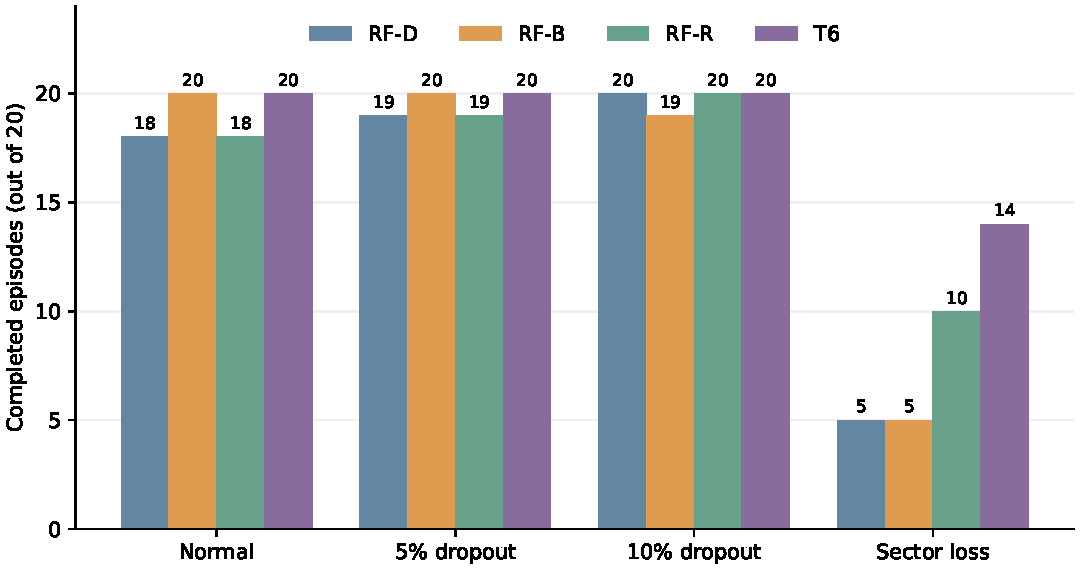
\includegraphics[width=\textwidth]{completion_by_condition.pdf}
\caption[Completion by sensor condition]{Completed episodes out of 20 per sensor condition, computed from
the four primary reports. Each condition aggregates four maps and five starts
per map; bars are descriptive counts, not independent-map reliability estimates.}
\label{fig:completion}
\end{figure}

The strongest offline accuracy belongs to RF-R, whereas the best primary
closed-loop completion count belongs to T6. This mismatch answers the central
comparison question: prediction accuracy alone does not rank these controllers
by their recorded driving outcomes. The student repeatedly selects its own
future observations during driving, whereas the offline data are teacher
trajectories. This distinction is consistent with the learner-induced state
distribution problem in sequential imitation~\cite{ross2011reduction}.
Model-selection decisions should therefore retain the two
levels of evidence rather than replace closed-loop testing with a single
classification score.

\section{Augmentation and Sensor Loss}
RF-B improves on RF-D by two completions in the primary matrix, but RF-R
completes more episodes than either. The observed data do not demonstrate a
consistent advantage from the chosen scattered-dropout augmentation. They
also do not show that augmentation is generally ineffective: the conclusion
concerns this masking rule, this training distribution and these model
configurations.

Forty-six of the 53 primary collision episodes occur in the sector condition.
Scattered loss preserves measurements across much of the visible region,
whereas a contiguous blind region can remove neighbouring directions at the
same time. The recorded outcomes are consistent with sensitivity to this
spatial difference. However, the per-step logs do not contain the original
scan or exact masking indices, so the study cannot identify a particular
missing angular segment as the demonstrated cause of each collision.

The primary matrices also show that an apparently easy map can mask an
important limitation. RF-D and RF-B both complete all five E2 sector episodes
but fail all five on each of the other three maps. Thus E2 sector success
cannot stand alone as evidence of robust operation across the evaluated
geometries.

\section{Repeated Runs and Training Seeds}
A second complete T6 matrix again records 74 completions and six collisions,
with a score of 89.10. An additional sector-only run again completes fourteen
of twenty episodes. RF-R's sector repeat decreases from ten completions to
eight. These repeats indicate both stable patterns and some sensitivity to
repeated execution under nominally matching settings.

Boundary repeats on R1 illustrate why small differences should be interpreted
carefully. RF-D changes from three of five normal completions in its primary
matrix to five of five in the repeat, while its dropout10 result changes from
five of five to three of five. RF-B changes from four to five dropout10
completions. Fixed seeds do not eliminate all runtime variation, but the
available logs do not establish a specific simulator or scan-timing cause.

Additional RF-B models trained with seeds 43 and 44 are evaluated on normal
and sector inputs only. Their normal completions are 20/20 and 19/20,
respectively; both complete 5/20 sector episodes. Seed 42 has 20/20 normal and
5/20 sector completions. These 40-episode subsets are not full 80-episode
matrices. T6 trained with seeds 42, 43 and 44 produces identical exported
headers, so the extra seed artifacts are not counted as three different
deployed tree policies or three new closed-loop experiments.

\section{Cross-Batch Offline Assessment}
The later batch is assessed without changing any fitted model.
Table~\ref{tab:crossbatch} reports equal-map averages across the four maps.
The corresponding project report is identified in Appendix~\ref{sec:evidence_analysis}.
Because three are fitting maps, these averages are not estimates of
unknown-map generalisation. They describe prediction on a later collection
with new starts and a different seed under the same map set.

\begin{table}[htbp]
\centering\small
\caption[Cross-batch offline assessment]{Later-batch offline metrics, averaged equally over four maps.
Macro F1 uses the fixed six-label set and zero for undefined class scores.}
\label{tab:crossbatch}
\begin{tabular}{lrrrr}
\toprule & \multicolumn{2}{c}{Raw} & \multicolumn{2}{c}{Dropout} \\
\cmidrule(lr){2-3}\cmidrule(lr){4-5}
Model & Accuracy & Macro F1 & Accuracy & Macro F1 \\\midrule
RF-D & .8522 & .4204 & .8495 & .4188 \\
RF-B & .8536 & .4210 & .8515 & .4196 \\
RF-R & .8569 & .4203 & .8553 & .4194 \\
T6 & .8530 & .5007 & .8471 & .4869 \\
\bottomrule
\end{tabular}
\end{table}

Under matching aggregation, the archived cross-batch comparison reports small
accuracy and MAE differences for most model/input combinations. This supports
consistency under the observed collection change, not an absence of all
possible distribution shifts. On later-batch E2 raw input, T6 has accuracy
about 0.666, compared with approximately 0.753--0.769 for the forests. Its
fixed-six-class F1 is nevertheless higher. That observation repeats the
metric-ranking distinction seen in the earlier validation.

Later-batch E2 contains thirteen label-5 samples and no label-12 samples.
Fixed-label F1 and present-class F1 therefore need separate interpretation.
Cross-batch changes in a macro score may reflect both predictions and changing
class support. The individual support counts are retained in the accompanying
analysis artifacts instead of attributing every aggregate change to improved
or degraded learning.

\section{Failure Cases and Interpretation}
Figure~\ref{fig:collisionmaps} shows the primary collision endpoints. The seven
non-sector collisions all occur on R1, at approximately 52.6--169.8~s.
Several terminate near similar bends at around 169~s and 33.8~m of travel.
This locates a recurrent difficult region, but does not by itself establish
whether the cause is scan timing, accumulated steering error or a particular
input partition.

\begin{figure}[htbp]
\centering\includegraphics[width=\textwidth]{r6_collision_map.png}
\caption[Collision endpoints on the evaluated maps]{Primary collision endpoints on the four maps, reproduced from the
archived failure analysis. Overlapping markers may represent multiple episodes.
Map coordinates are in metres.}
\label{fig:collisionmaps}
\end{figure}

Successful sector episodes contain more total action switches than early
collision episodes. Since successful episodes run for longer, raw switching
counts are confounded by exposure time. A claim that rapid corrections cause
success would require switching rates or aligned trajectory windows, together
with the relevant observations. The current evidence supports a description
of the action sequences, not this causal explanation.

Likewise, the higher rare-class recall of T6 is a possible contributor to its
behaviour, but the comparison changes several model properties simultaneously.
The appropriate conclusion is that the tested T6 configuration is a stronger
candidate under the current matrix. Isolating depth, feature sampling or
ensemble effects requires additional matched comparisons.

\section{Implications for the Proposed Training Strategy}
The forest results show that teacher-generated supervision can produce useful
LiDAR-only driving without human-labelled trajectories in this pipeline. The
single-tree result shows why the research objective must remain broader than
confirming an initial model preference: a simpler tested student can retain
more useful closed-loop behaviour than the selected shallow ensembles. This
favours further investigation of T6 while preserving the role of the forests
as the principal design candidates and data-variant comparisons.

The result also constrains the automation claim. The teacher's collection
coverage and the student's representation determine which situations are learnt.
Large quantities of cruising data do not automatically cover states caused by
student errors or contiguous sensor loss. Additional automated data should
therefore be directed at a demonstrated gap, with its effects evaluated in
closed loop, rather than assuming that more simulation alone solves the problem.

No matched human-labelled training baseline or physical power measurement is
available. The evidence supports an alternative source of supervision and
candidate compact policies; it does not yet quantify savings in labour or energy.

\section{Limitations and Outstanding Evaluation}
Each map/condition cell has only five starts, and repeated starts on the same
four maps do not establish a broad distribution of environments. Correlated
frames, paired augmentations and identical exported policies must not be
counted as independent replication. Aggregate counts in this chapter are
therefore descriptive; no statistical significance claim is made.

The independent-map and student recovery experiment remains pending. Its
planned base design comprises two frozen models, two new maps, three start
classes and five episodes per cell, giving 60 episodes. A further 40 episodes
would evaluate dropout10 and sector conditions from normal starts on the new
maps. These are proposed measurements, not results. Teacher near-wall
collection cannot fill the missing student-recovery evidence.

Finally, the evaluated policies depend on a fixed forward speed, a limited
action set and a single scan. Wider tasks involving reverse motion, dynamic
obstacles or route planning have not been tested. Host export agreement does
not establish physical timing or safety. These boundaries allow the completed
simulation findings to be used without extending them to unsupported claims.
